\documentclass
[handout]
{beamer}
\usepackage{hyperref}

%%
%%
%%
% From http://tex.stackexchange.com/questions/2072/beamer-navigation-circles-without-subsections
% Solution #2 or 3:
% \usepackage{etoolbox}
% \makeatletter
% % replace the subsection number test with a test that always returns true
% \patchcmd{\slideentry}{\ifnum#2>0}{\ifnum2>0}{}{\@error{unable to patch}}%
% \makeatother
% Solution #1:
\usepackage{remreset}% tiny package containing just the \@removefromreset command
\makeatletter
\@removefromreset{subsection}{section}
\makeatother
\setcounter{subsection}{1}


\usepackage{etex}
\usepackage{pgf}
\usepackage{tikz}
\usepackage{url}
\usepackage{amsmath}
\usepackage{color}
% \definecolor{red}{rgb}{1,0,0}
\usepackage{ulem}
% \usepackage{booktabs}
\usepackage{colortbl,booktabs}
\renewcommand*{\thefootnote}{\fnsymbol{footnote}}
\usepackage{fancybox}
\usepackage[framemethod=TikZ]{mdframed}
\mdfdefinestyle{FactStyle}{%
  outerlinewidth=0.5,
  roundcorner=1pt,
  leftmargin=1cm,
  linecolor=blue,
  outerlinecolor=blue!70!black,
  backgroundcolor=yellow!40
}
\usepackage{cancel}

  \newcommand\Warning{%
    \makebox[2.4em][c]{%
      \makebox[0pt][c]{\raisebox{.2em}{\Large!}}%
      \makebox[0pt][c]{\color{red}\Huge$\bigtriangleup$}}}%

\usepackage{stackengine}
\usepackage{scalerel}
\usepackage{xcolor}
  \newcommand\dangersign[1][2ex]{%
    \renewcommand\stacktype{L}%
    \scaleto{\stackon[1.3pt]{\color{red}$\triangle$}{\tiny !}}{#1}%
  }



\usepackage{dcolumn}
\newcolumntype{d}[1]{D{.}{.}{#1}}

% From
% http://tex.stackexchange.com/questions/109900/how-can-i-box-multiple-aligned-equations
\usepackage{empheq}
\usepackage{tcolorbox}  \newtcbox{\othermathbox}[1][]{%
  nobeforeafter, tcbox raise base, 
  colback=black!10, colframe=red!30, 
  left=1em, top=0.5em, right=1em, bottom=0.5em}

\newcommand\blue{\color{blue}}
\newcommand\red{\color{red}}
\newcommand\green{\color{green!75!black}}
\newcommand\purple{\color{purple}}
\newcommand\bluegreen{\color{blue!75!green}}
\newcommand\orange{\color{orange}}
\newcommand\redgreen{\color{red!50!green}}
\newcommand\grey{\color{black}}
\newcommand\gap{\vspace{.1in}}
\newcommand\nb{${\red\bullet}\ $}
\newcommand\halfgap{\vspace{.05in}}
\newcommand\divideline{\line(1,0){352}}
\usepackage{marvosym} % for \Smiley

\newcommand{\bluealert}[1]{{\blue\textbf{#1}}}

% \usepackage{beamerthemesplit} %Key package for beamer
\usetheme{Singapore}
% \usetheme{Szeged}
% \usetheme{Garfield}
% \usetheme{CambridgeUS}
% \usenavigationsymbolstemplate{} %Gets rid of slide navigation symbols


\setbeamercolor{separation line}{use=structure,bg=structure.fg!50!bg}
% \begin{beamercolorbox}[colsep=0.5pt]
%   {upper separation line foot}
% \end{beamercolorbox}



\makeatletter
\setbeamertemplate{footline}
{
  \leavevmode%
  \hbox{%
% \begin{beamercolorbox}[colsep=0.5pt]
%   {upper separation line foot}
% \end{beamercolorbox}


  \begin{beamercolorbox}[wd=.5\paperwidth,ht=2.25ex,dp=2ex,colsep=0.5pt]%
    {upper separation line foot}
    \usebeamerfont{author in head/foot}%
    \hspace*{2ex}\insertshortdate:\ \insertshorttitle
  \end{beamercolorbox}%
  \begin{beamercolorbox}[wd=.5\paperwidth,ht=2.25ex,dp=2ex,right]{title in head/foot}%
    \usebeamerfont{title in head/foot}
    {\insertshortauthor}\hspace*{2ex}
  \end{beamercolorbox}}%
  % \begin{beamercolorbox}[wd=.333333\paperwidth,ht=2.25ex,dp=2ex,right]{date in head/foot}%
  %   \usebeamerfont{date in head/foot}\insertshortdate{}\hspace*{2em}
  %   \insertframenumber{} / \inserttotalframenumber\hspace*{2ex} 
  % \end{beamercolorbox}%
  \vskip0pt%
}
\makeatother

\usetikzlibrary{decorations.markings}
\usetikzlibrary{arrows}


\title{Final Exam Review}
\author{Peter Garfield, UCSB Mathematics}
\date{March 15, 2017}
%\institute{}


\useinnertheme{default}

\usefonttheme{serif}
% \usecolortheme{rose}
% \usecolortheme{whale}
% \usecolortheme{orchid}
\usecolortheme{crane}
% \usecolortheme{dolphin}


%TEMPLATE
\setbeamertemplate{navigation symbols}{}

\setbeamertemplate{note page}[compress]

\setbeamertemplate{frametitle}{
  \vspace{0.5em}
  % \begin{centering}
  {\huge\blue\textbf{\textmd{\insertframetitle}}}
  \par
  % \end{centering}
}

% From http://tex.stackexchange.com/questions/7032/good-way-to-make-textcircled-numbers:
\newcommand*\circled[1]{\tikz[baseline=(char.base)]{\node[shape=circle,draw,fill=orange,inner sep=1pt] (char) {#1};}} 
% \renewcommand{\labelenumi}{\circled{\textbf{\arabic{enumi}}}}

\let\olddescription\description
\let\oldenddescription\enddescription
\usepackage{enumitem}
\let\description\olddescription
\let\enddescription\oldenddescription

% \usepackage[loadonly]{enumitem}
\setlist[enumerate,1]{label=\colorbox{orange}{\arabic*.},font=\bfseries}
%\setlist[enumerate,2]{label=\colorbox{blue!25}{(\alph*)},font=\bfseries}
% \setlist[enumerate,1]{label=\arabic*.,font=\bfseries}
\setlist[itemize,1]{label=\red$\bullet$}
\setlist[itemize,2]{label=\blue$\bullet$}

\newcommand\answer[1]{\fbox{#1}}
% \renewcommand\answer[1]{}

\newcommand{\antilog}{\operatorname{antilog}}







\title{Units, Areas \& Volumes}
\author{Trevor Klar, UCSB Mathematics}
\date{June 23, 2022}


\begin{document}
\section{Introduction}

\frame{
  \frametitle{}
  {\Huge{}Welcome To Math 34A!}\\[.5em]

  {\Huge{}Differential Calculus}
  \vfill
  {\Large{}Instructor:}\\
  \ \hspace*{0.2in} Trevor Klar, \url{trevorklar@math.ucsb.edu}\\
  \ \hspace*{0.2in} South Hall 6431X (Grad Tower, 6th floor, blue side, first door on the right)
  \\[0.5em]

  {\Large{}Office Hours:}\\
  \ \hspace*{0.2in} MTWR after class 2:00-3:00, and by appointment. Details on Gauchospace. 
  \bigskip

  {\tiny \copyright\ 2017-22\ Daryl Cooper, Peter Garfield, Ebrahim Ebrahim, Nathan Schley, and Trevor Klar}\\
  Please do not distribute outside of this course.
  \vfill

}

%Notetaker%%%%%%%%%%%%%%
% \frame{
%   \frametitle{DSP Notetaker Needed}

%   If you are interested in earning \$25 per unit by taking notes for a student in need, please apply online: \vspace{.4in} \\ 
%   {\blue \url{http://dsp.sa.ucsb.edu/services}} \vspace{4pt} \\ 
%   Questions: {\red \url{notes@sa.ucsb.edu}} \vspace{.4in} \\ 
%   (These slides will be posted on Gauchospace, so you can click the link there for convenience). 

% }





\section*{Pythagorean Theorem}

\small
\frame{
  \frametitle{\S1.7: Pythagoras' Theorem}

  \begin{minipage}{0.4\linewidth}
    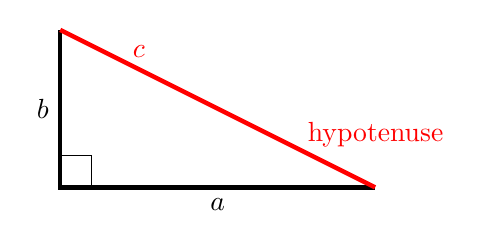
\begin{tikzpicture}[x=10mm,y=10mm,>=latex]
      \draw[ultra thick,black] (0,2) -- (0,0) node[midway,left] {$b$} -- (4,0) node[midway,below] {$a$};
      \draw[ultra thick,red] (0,2) -- (4,0) node[near start, above] {$c$} node[near end, right,
yshift=0.5em] {hypotenuse};
      \draw[thin,black] (0.4,0) -- (0.4,0.4) -- (0,0.4);
    \end{tikzpicture}
  \end{minipage}
  \begin{minipage}{0.55\linewidth}
    \begin{empheq}[box=\othermathbox]{align*}
      c^2 
      & = a^2 + b^2
    \end{empheq}
  \end{minipage}

  \begin{enumerate}
    \setcounter{enumi}{10}
  \item  What is the length of the hypotenuse of a right triangle when
    the other two sides have length ${\blue 3}$ and ${\blue 4}$? 

    \begin{center}
      A $=3$
      \quad 
      B $=4$
      \quad 
      C $=6$
      \quad 
      D $=25$
      \quad 
      E $=\text{none of these}$
      \pause 
      \quad
      \answer{E}
    \end{center}
    % They hypotenuse is length $5$!
    \smallskip
    \pause

  \item Now lengths are ${\blue 2}$ and ${\blue 3}$.  What's the hypotenuse?
    \begin{center}
      A $=\sqrt{5}$
      \quad 
      B $=\sqrt{13}$
      \quad 
      C $=13$
      \quad 
      D $=5$
      \pause
      \quad
      \answer{B}
    \end{center}
    \smallskip
    \pause

  \item Lengths ${\blue 3x}$ and ${\blue 4x}$. What's the hypotenuse?
    \begin{center}
      A $=5+x$
      \quad 
      B $=5x^2$
      \quad 
      C $=25x$
      \quad 
      D $=5x$
      \pause
      \quad
      \answer{D}
    \end{center}
  \end{enumerate}
  % This is \colorbox{yellow}{very useful}.

}


\frame{
  \frametitle{Pythagorean Theorem Applications}

  This is \colorbox{yellow}{very useful}\ to calculate how far apart two things are.
  \bigskip

  \begin{enumerate}
    \setcounter{enumi}{13}
  \item You and Marie are in Vegas. You drive north at 40 mph and
    Marie drives east at 30 mph.  How far apart are you after 1 hour?

    Click A when you have the answer.
    \pause
    \bigskip

  \item How many miles apart are you after $t$ hours? 
    \begin{center}
      A $= 50t$
      \quad 
      B $= 50+t$
      \quad 
      C $= 50t^2$
      \quad 
      D $= 2500t^2$
      \quad
      \pause
      \answer{A}
    \end{center}
    \bigskip
  \end{enumerate}


}

\frame{
  \frametitle{A word problem to start off}

  \begin{enumerate}
    \setcounter{enumi}{0}
  \item The vertical mast of a yacht is $40$ feet high. A rope runs in
    a straight line from the top to a pulley $30$ feet horizontally
    from the base of the mast. How many feet long is the rope?

    \textbf{Hint:}\ Draw a picture!

    \begin{center}
      A $=30$
      \quad 
      B $=40$
      \quad 
      C $=50$
      \quad 
      D $=60$
      \quad 
      E $=70$
      \quad
      \pause
      \answer{C}
    \end{center}
  \end{enumerate}
  \vspace{2in}
}

\frame{
  \frametitle{Why Pythagorean Theorem works}

\begin{center}
  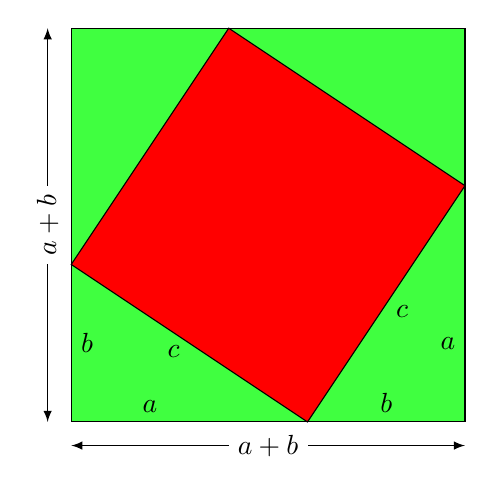
\begin{tikzpicture}[x=10mm,y=10mm,>=latex]
    \draw[thin,black,<->] (0,-3mm) -- (5,-3mm) node[midway,fill=white] {$a+b$};
    \draw[thin,black,<->] (-3mm,0) -- (-3mm,5) node[midway,fill=white,rotate=90] {$a+b$};
    \draw[thin,black,fill=green!75] (0,0) rectangle (5,5);
    \draw[thin,black,fill=red] (0,2) -- (3,0) -- (5,3) -- (2,5) -- cycle;
    % Bottom left:
    \node[above] at (1,0) {$a$};
    \node[right] at (0,1) {$b$};
    \node[left,yshift=-1mm] at (1.5,1) {$c$};
    % Bottom right:
    \node[left] at (5,1) {$a$};
    \node[above] at (4,0) {$b$};
    \node[right,yshift=-1mm] at (4,1.5) {$c$};
  \end{tikzpicture}
  % \includegraphics[scale=0.5]{PythagorasProofSmall.pdf}
\end{center}


% area of big square $= (a+b)^2$\\
% area of each green triangle $=\green ab/2$\\
% area red square $=c^2$\\

% area of big square is ${\red c^2} + 4({\green ab/2}) = (a+b)^2$\\
% simplify $c^2 + 2ab = a^2 + 2ab +b^2\quad\Rightarrow\quad$ \fbox{$c^2=a^2+b^2$}

}

\section*{Area \& Volume}

\frame{
  \frametitle{\S4.2: Area and Volume}

  You need to know:
  \begin{itemize}
  \item Area of a rectangle = length $\times$ width

  \item Area of a circle = $\pi R^2$\qquad ($R= \text{radius})$

  \item Circumference of a circle = $2\pi R$

  \item Area of a triangle = half base $\times$ height $=\dfrac{1}{2}
    b h$

  \item volume of rectangular box = (length $\times$ width) $\times$ height\\
    \hspace*{1.58in} = (area of {\red base}) $\times$ height
    % \phantom{volume of rectangular box} = (area of {\red base}) $\times$ height

  \end{itemize}

  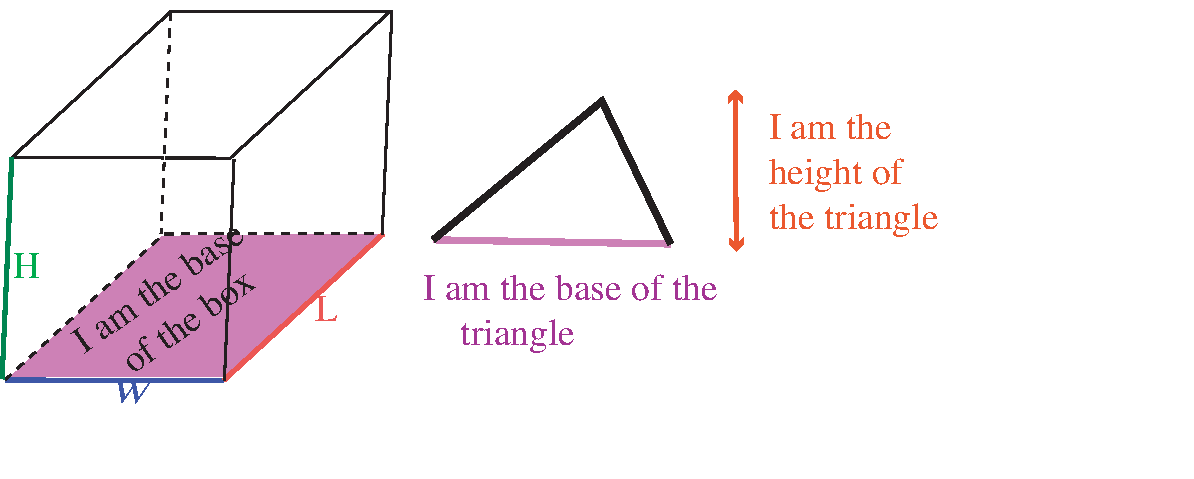
\includegraphics[scale=0.3]{L4basesmallnew}\quad
  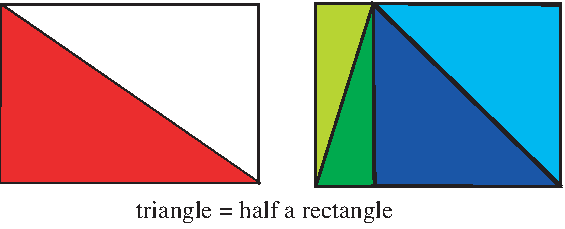
\includegraphics[scale=0.45]{trianglehalfrectanglesmall}

}

\frame{

What is the (circumference of a circle) divided by the diameter?
\begin{center}
  $A=R$
  \quad 
  $B=2\pi$
  \quad 
  $C = \pi$
  \quad 
  $D=$the what now?
  \quad
  \pause
  \fbox{C}
\end{center}
\pause 

The definition of $\pi$ is 
\begin{equation*}
  \pi 
  = \frac{\text{circumference of circle}}{\text{diameter}}
  \pause
  = \frac{C}{2R},
\end{equation*}
\pause
so $C = 2\pi R$.
\vspace*{-0.5in}

\gap
\begin{center}
  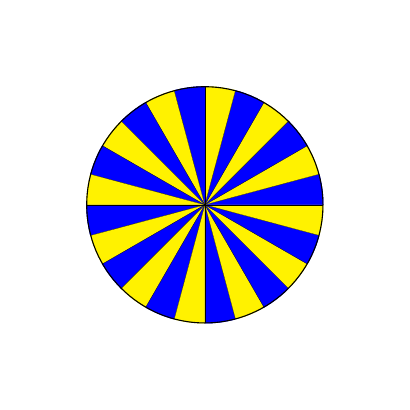
\begin{tikzpicture}[x=15mm,y=15mm,>=latex]
    \foreach \theta in {0,30,60,...,330}
    {
      \begin{scope}
        \clip ({1.5*cos(\theta)},{1.5*sin(\theta)}) -- (0,0) -- ({1.5*cos(15+\theta)},{1.5*sin(15+\theta)}) -- cycle;
        \filldraw[blue] (0,0) circle (1);
      \end{scope}
      \begin{scope}
        \clip ({1.5*cos(30+\theta)},{1.5*sin(30+\theta)}) -- (0,0) -- ({1.5*cos(15+\theta)},{1.5*sin(15+\theta)}) -- cycle;
        \filldraw[yellow] (0,0) circle (1);
      \end{scope}
    }
    \foreach \theta in {0,30,60,...,330}
    {
      \draw[ultra thin,black] (0,0) -- ({cos(\theta)},{sin(\theta)});
      \draw[ultra thin,black] (0,0) -- ({cos(15+\theta)},{sin(15+\theta)});
    }
    \draw[thin,black] (0,0) circle (1);
  \end{tikzpicture}
  \hspace*{0.01in}
  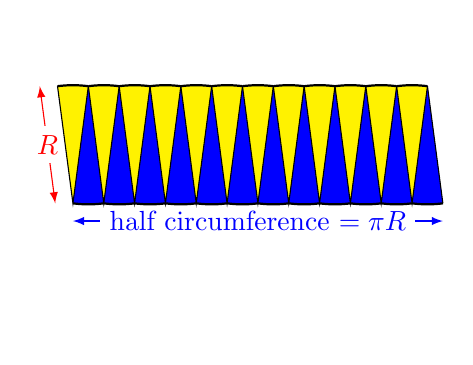
\begin{tikzpicture}[x=15mm,y=15mm,>=latex,baseline=-17mm]
    \draw[thin,red,<->] ({-1*cos(82.5)-0.15},{sin(97.5)}) -- (-0.15,0) node[midway,fill=white] {$R$};
    \draw[thin,blue,<->] (0,-0.15) -- ({24*cos(82.5)},-0.15) node[midway,fill=white] {half circumference $=\pi R$};
    \foreach \k in {0,1,2,...,11}
    {
      \begin{scope}
        \clip ({2*\k*cos(90-7.5)+1.5*cos(90-7.5)},{1.5*sin(90-7.5)}) -- ({2*\k*cos(90-7.5)},0) -- ({2*\k*cos(90-7.5)+1.5*cos(90+7.5)},{1.5*sin(90+7.5)}) -- cycle;
        \draw[thick,black,fill=yellow] ({2*\k*cos(90-7.5)},0) circle (1);
      \end{scope}
      \begin{scope}
        \clip ({(1+2*\k)*cos(90-7.5)+1.15*cos(90-7.5)},{sin(90-7.5)-1.15*sin(90-7.5)}) -- ({(1+2*\k)*cos(90-7.5)},{sin(90-7.5)}) -- ({(1+2*\k)*cos(90-7.5)+1.15*cos(90+7.5)},{sin(90-7.5)-1.15*sin(90+7.5)}) -- cycle;
        \draw[thick,black,fill=blue] ({(1+2*\k)*cos(90-7.5)},{sin(90-7.5)}) circle (1);
      \end{scope}
    }
    \foreach \k in {0,2,...,23}
    {
      \draw[thin,black] ({(\k-1)*cos(82.5)},{sin(97.5)}) -- ({\k*cos(82.5)},0) -- ({(\k+1)*cos(82.5)},{sin(97.5)});
    }
    \draw[thin,black] ({23*cos(82.5)},{sin(97.5)}) -- ({24*cos(82.5)},0);
  \end{tikzpicture}
\end{center}
\vspace*{-0.5in}
\pause
\gap
\ \hfill \fbox{Thus Area$=({\red R})({\blue\pi R})=\pi R^2$}\hfill\ 


}


% taken from L5
\frame{
  \frametitle{Applications}
  \begin{enumerate}
    \setcounter{enumi}{1}
  \item A rectangular  parking lot is to be made in the shape of a rectangle.
    It will have an area of {\purple 2000} square meters.
    Express the {\blue length} of the parking lot in terms of the
    {\red W = width}.

    \begin{center}
      A $= (2000-2W)/2$
      \quad 
      B $= 2000/W$
      \quad 
      C $= 2000-W$
      \\[0.5em]
      D $=\text{Other}$
      \quad
      \pause
      \answer{B}
    \end{center}
    \smallskip
    \pause

  \item The parking lot will be surrounded by a fence. Express the
    {\blue total length of the fence} in terms of $W$.

    \begin{center}
      A $= 2000+2W$
      \quad 
      B $=L+W$
      \quad 
      C $= 4000W^{-1}+ 2W$
      \quad
      \pause
      \answer{C}
    \end{center}
    \pause
    \smallskip

  \item The fence costs \$7 per meter.  Express the total cost of all
    the fence in terms of $W$. 
    \begin{center}
      A $= 7\times 2000$
      \quad 
      B $= 7\times 4000W^{-1}+2W$
      \\[0.5em]
      C $= 28000W^{-1}+14W$
      \quad
      \pause
      \answer{C}
    \end{center}

  \end{enumerate}

}


\frame{
  \frametitle{Applications II}

  \begin{enumerate}
    \setcounter{enumi}{4}
  \item A rectangular poster is to have a total area of
    $500\ \text{cm}^2$.  There is an empty margin where nothing is
    printed $6$ cm wide at the top and $4$ cm wide along the sides and
    bottom. The rest is the printed area.

    \textbf{Hint:}\ Draw a picture! Name your unknowns!

    % \includegraphics[scale=0.4]{L4pic2small}
    % \uncover<3->{\qquad\qquad\includegraphics[scale=0.45]{L4pic3small}}

    \begin{itemize}
    \item Express printed area in terms of width $W$ and height $H$ of the poster.

      \begin{center}
        A $=HW$
        \quad 
        B $=(H-8)(W-8)$
        \quad 
        C $=\text{Other}$
        \qquad
        \pause
        \answer{C}
      \end{center}
      \bigskip
        \pause

    \item Express the area of the printed part in terms of the width
      $W$ of the poster.
    \begin{center}
      A $= \text{got it!}$
      \quad 
      B $= \text{working on it}$
      \qquad
      C $= \text{help}$
    \end{center}
    \textbf{Hint:}\ Express $H$ in terms of $W$.
    \bigskip

    \end{itemize}
  \end{enumerate}

}


\frame{

{\purple 3.2.41} Express the {\orange total surface area} of a cube in terms of its {\blue volume V}.\\

Draw a picture! Name the unknowns!
\gap

\uncover<2->{%
{\vspace*{-4em}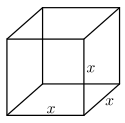
\includegraphics[scale=0.35]{L4cubesmall}}\quad\uncover<3->{\parbox[b]{81mm}{%
  \vspace*{3.5em}
  ${\red x}$ = length of one side of cube\\[.25em]
  (area of each side) = \ \ \ ${\red x}^2$\\[.25em]
  There are 6 sides so\\[.25em]
  \fbox{{\orange total surface area} = $6{\red x}^2$}%$\cdots\cdots$\fbox{1}
  \vspace*{1em}
}}
}

\uncover<2->{%
  {\green Plan:} \\
  As a first step find {\orange total  area} in terms of {\red x}\\

  {\orange total surface area} is\quad
  $A={\red x}^2\quad B=6{\red x}\quad C={\red x}^3\quad D=6{\red x}^3\quad E=6{\red x}^2$
  \quad\uncover<3->{\fbox{E}}
}

\halfgap
\pause\pause\pause Now express  {\red x} in terms of  {\blue V}  \\ \pause
{\blue V} = volume of cube = ${\red x}^3$ so solve for {\red x}\\ \pause
 ${\red x}=\sqrt[3]{\blue V}$\\ \pause
 sub for ${\red x}$ in \fbox{1} get  {\orange total surface area} = \fbox{$6(\sqrt[3]{{\blue V}})^2$}


}




\section*{Units!}

\frame{
  \frametitle{Units: A Meaningless Calculation}

  \begin{center}
    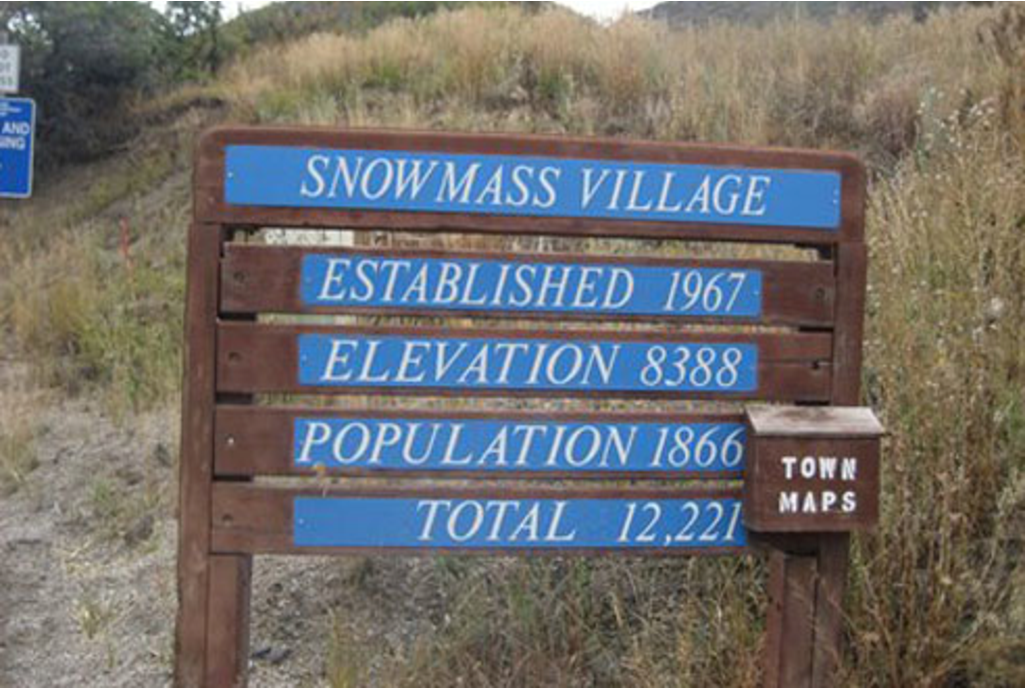
\includegraphics[scale=0.6]{Snowmass}
  \end{center}
}
   
\frame{
  \frametitle{Units: A Meaningless Calculation}

  \alert{Rule:}\ Only \alert{add or subtract}\ things measured in \emph{same units}\\ \pause
  \begin{itemize}
  \item  3 meters + 7 inches is NOT 10 of {\blue anything} \pause
  \item 2 days + 5 hours $\ne 7$ \pause
  \item 3 nickels + 2 dimes $\ne$ 5\pause
  \end{itemize}
  
  \gap
  \alert{BUT!}\ You \emph{can multiply or divide things}\ in different units:
  
\begin{center}  \fbox{average speed = (distance gone)/(time taken)}\end{center}
  
(50 {\green miles}){\blue /}(1 {\green hour}) = 50 ({\green miles{\blue /}hours}) = 50 {\green miles {\blue per} hour} = 50 {\green m{\blue p}h}\\
  You must {\blue multiply or divide} the {\green units} too !\\ \pause
  {\green miles} {\blue divided} by {\green hours} is {\green miles {\blue per} hour}

}

\frame{

  When a problem has {\red mixed units} like {\green miles and feet}
  or {\purple years and seconds} {\red decide} what units you will use
  (like {\orange miles} and {\purple seconds}) and convert everything
  into those units, or\
  \pause 
  \begin{center}
    \colorbox{yellow}{{\red\Huge\textsf{SUFFER}}}
  \end{center}
  \pause


  \alert{\large{}Units conversions}

  \begin{enumerate}
    \setcounter{enumi}{5}
  \item How fast does your hair grow\ldots\pause{}in mph?
  \pause
    \begin{center}
      A$=10^{-3}$
      \quad
      B$=10^{-4}$
      \quad
      C$=10^{-5}$
      \quad
      D$=10^{-6}$
      \quad
      E$=10^{-8}$
      \quad
      \pause\fbox{???}
    \end{center}
    \pause
    I don't know either.
    \gap
   \pause
  \item How fast does your hair grow\ldots\pause{}in $\text{cm}/\text{month}$?
  \pause
    \begin{center}
      A$=$faster
      \quad
      B$=10$
      \quad
      C$=1$
      \quad
      D$=1/10$
      \quad
      E$=$slower
      \quad
      \pause\fbox{C}
    \end{center}
  \end{enumerate}

  \alert{\large{}Conversions:}
  \begin{equation*}
    2.54\ \text{cm} = 1\ \text{inch}
    \qquad
    12\ \text{inches} = 1\ \text{foot}
    \qquad
    5280\ \text{feet} = 1\ \text{mile}
  \end{equation*}
  \begin{equation*}
    30\ \text{days} = 1\ \text{month}
    \qquad
    24\ \text{hours} = 1\ \text{day}
  \end{equation*}

}

\frame{

\gap

  \begin{tabular}{ccccc}
    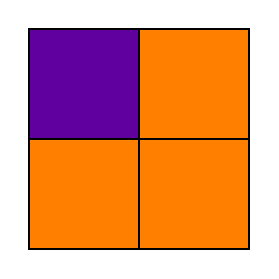
\begin{tikzpicture}[x=14mm,y=14mm,>=latex,baseline=0]
      \draw[thick,black,fill=orange] (0,0) rectangle (1,1);
      \draw[thick,black,fill=orange] (0,0) rectangle (1,-1);
      \draw[thick,black,fill=orange] (0,0) rectangle (-1,-1);
      \draw[thick,black,fill=purple!50!blue] (0,0) rectangle (-1,1);
    \end{tikzpicture}
    & \hspace*{0.25in}
    &
    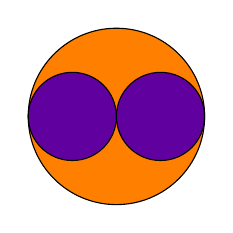
\begin{tikzpicture}[x=14mm,y=14mm,>=latex,baseline=0]
      \draw[thin,black,fill=orange] (0,0) circle (0.8);
      \draw[thin,black,fill=purple!50!blue] (-0.4,0) circle (0.4);
      \draw[thin,black,fill=purple!50!blue] (0.4,0) circle (0.4);
    \end{tikzpicture}
    & \hspace*{0.25in}
    &
    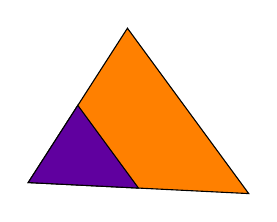
\begin{tikzpicture}[x=14mm,y=14mm,>=latex,baseline=-6mm]
      \draw[thin,black,fill=orange] (-1,-0.9) -- (1,-1) -- (-0.1,0.5) -- cycle;
      \draw[thin,black,fill=purple!50!blue] (-1,-0.9) --
      ({-1+0.5*2},{-0.9+0.5*(-0.1)}) --
      ({-1+0.5*(0.9)},{-0.9+0.5*1.4}) -- cycle;
    \end{tikzpicture}
    \\[4em]
    \parbox{28mm}{The\ {\color{orange}large square}\ is $2$ times the
    base of the {\color{purple!50!blue}small square}.  It has $2\times
    2= 4$ times the area.}
    &&
    \parbox{28mm}{The\ {\color{orange}large circle}\ is $2$ times the
    size of the {\color{purple!50!blue}small circle}.  It has $4$
      times the area.} 
    &&
    \parbox{28mm}{The\ {\color{orange}large triangle}\ is $2$ times the
    size of the {\color{purple!50!blue}small triangle}.  It has $4$
       times the area.} 
  \end{tabular}
  \gap
  \pause

  When you {\red double} the size of a shape the {\blue area} is multiplied by {\blue 4}\\ \pause
  \smallskip

  If you make a shape {\blue 3} times larger the area is {\blue 9} times as much\\ \pause
  \smallskip

  $\red x$ times larger gives {$\red {x}^{\blue 2}$} times as much area \pause
  % \smallskip

  \begin{empheq}[box=\othermathbox]{align*}
    \text{ area grows as {\blue the square} of the linear dimensions}
  \end{empheq}


  \begin{center}
  \end{center}


}

\frame{

  \begin{empheq}[box=\othermathbox]{align*}
    \text{When you {\red double} the size of a solid object,}\\
    \text{the volume is {\blue 8} times as much}\qquad\quad
  \end{empheq}
  \gap
  What is going on?\pause

  \halfgap
  An area has {\blue two dimensions} : {\red length} and {\red width}. \\
  Both of these get doubled so area is doubled {\purple twice} so multiplied by $2^{\blue 2}$\pause

  \gap A solid object has {\blue three dimensions} : {\red length, width} and {\red height}.\\
  Each dimension is doubled so volume  doubled {\purple three times} : multiplied by $2^{\blue 3}$
  \pause

  Make a solid object $\red x$ times bigger, volume is {${\red x}^{\blue 3}$} times as much.\pause
  \begin{empheq}[box=\othermathbox]{align*}
    \text{volume grows as {\blue the cube} of the linear dimensions}
  \end{empheq}
  \pause


  {\blue Conclusion} Volume and area grow at {\red different rates}\\
  As you make an object bigger the volume gets bigger faster ({\blue cubing}) than the area (only {\blue squaring}).
  Opposite effect when you make it smaller: volume gets smaller faster than area.



}

\frame{
  \frametitle{Consequences!} % of: Volume and area grow at different rates}

  \alert{Many important consequences} read {\purple section 4.4}
  \bigskip

  Why do babies get cold faster than adults?\\ 
  Why can an ant pick up something weighing 10 times its own weight?\\ 
  Why are humans 60 feet tall  {\blue mathematically impossible}?\\
  Why can't you build a jumbo jet twice as big?\\
  Why are my lungs crinkly?\\
  A planet made of rock behaves like a liquid\\
  Why can a fly walk on the ceiling, but I cant?\\
  Why is water so dangerous to an insect but not gravity?\\
  \pause
  \gap 

  Paraphrasing {\orange J.B.S.Haldane}\quad Falling down a {\red thousand yard mine shaft}\\
  A mouse  {\blue walks away}\\
  \pause
  A rat is {\blue killed}\\
  \pause
  A man is {\blue broken}\\
  \pause
  A horse {\blue splashes}
}

\frame{
  \begin{enumerate}
    \setcounter{enumi}{7}
  \item An oil leak!
    \begin{itemize}
    \item  Oil is leaking from an oil tanker at the rate of {\blue 4000} liters per hour.
    \item {\orange 8} liters of oil spread out over {\red 10} square meters of ocean surface.
    \item A {\purple SQUARE} oil slick forms. 
    \end{itemize}
    \vspace{1em}
    \begin{itemize}
    \item Express the length, $X$,  of one side of the square  oil
      slick as a function of the time $t$ (in hours) the tank has been
      leaking. 
    \item After {\blue how many hours} will the oil slick be a square
      with side length 2 kilometers?  
    \end{itemize}
  \end{enumerate}
  \pause

  {\blue PLAN:} 
  \begin{itemize}
  \item[(i)] How many liters of oil on ocean  after $t$ hours?

  \item[(ii)] How much area does this oil cover?
  \end{itemize}
  \pause
  \gap

  {\blue Answer: \answer{$t=800\ \text{hours}$}}
}



\section*{Review}



\frame{
  \frametitle{Exercise}

  \begin{enumerate}
    \setcounter{enumi}{8}
  \item When you substitute $x = y+3$ into $x^2- 6x+8$ you get\ldots
    \begin{center}
      A $=y^2-6y-1$
      \quad 
      B $= y^2 + 35$
      \quad 
      C $=y^2-6 y+35$
      \quad 
      D $=y^2 -1$
      \quad
      \pause
    \end{center}
    \alert{Answer:}\ \answer{D}
    \pause
    \bigskip

  \item Can you check your answer to the previous question?
    \pause

    \textbf{Hint:}\ What are the expressions when $y = 1$? \\ 
    \pause 
    What is $x$ when $y=1$? 
    \pause

    When $y=1$, $x=4$ so $x^2 - 6x + 8 = 4^2 - 6(4)+8 = 0$.
    \pause

    The other expressions are\ldots
    \begin{center}
      A $=y^2-6y-1 = -6$
      \qquad \qquad 
      B $= y^2 + 35 = 36$
      \\[1em]
      C $=y^2-6 y+35 = 30$
      \qquad \qquad 
      D $=y^2 -1 = 0$
    \end{center}
    



  \end{enumerate}

}
 


\frame{
  \frametitle{That's it. Thanks for being here. }

  \begin{center}
    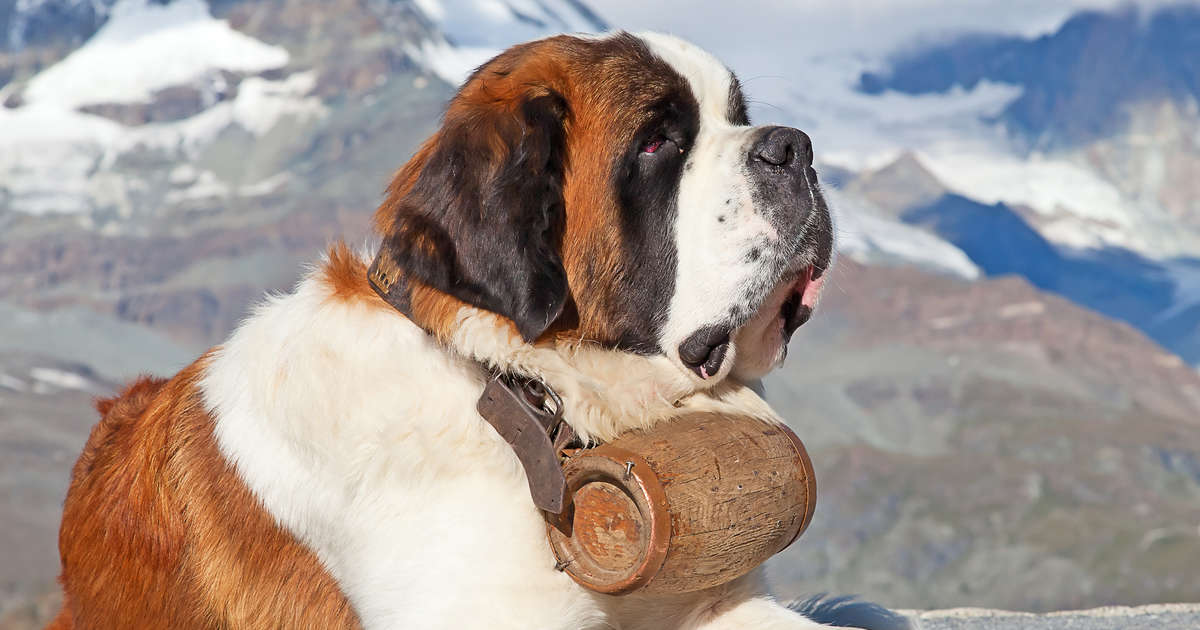
\includegraphics[scale=1]{Lecture 3 Picture.jpg}
  \end{center}
}





\end{document}


%%% Local Variables: 
%%% mode: latex
%%% TeX-master: t
%%% End: 
